% =====================================================================
%  Figure captions for
%  "The Directional Pair: A Model Without Identity, a Catalogue Without
%   Process, and the Single Table They Jointly Evaluate"
%
%  Every quantity quoted below is a measured value read from the executed
%  validation suite (validation/results/*.json).  Panels are generated by
%  validation/generate_panels.py.
% =====================================================================


% ---------------------------------------------------------------------
%  PANEL 1
% ---------------------------------------------------------------------
\begin{figure*}[!htbp]
    \centering
    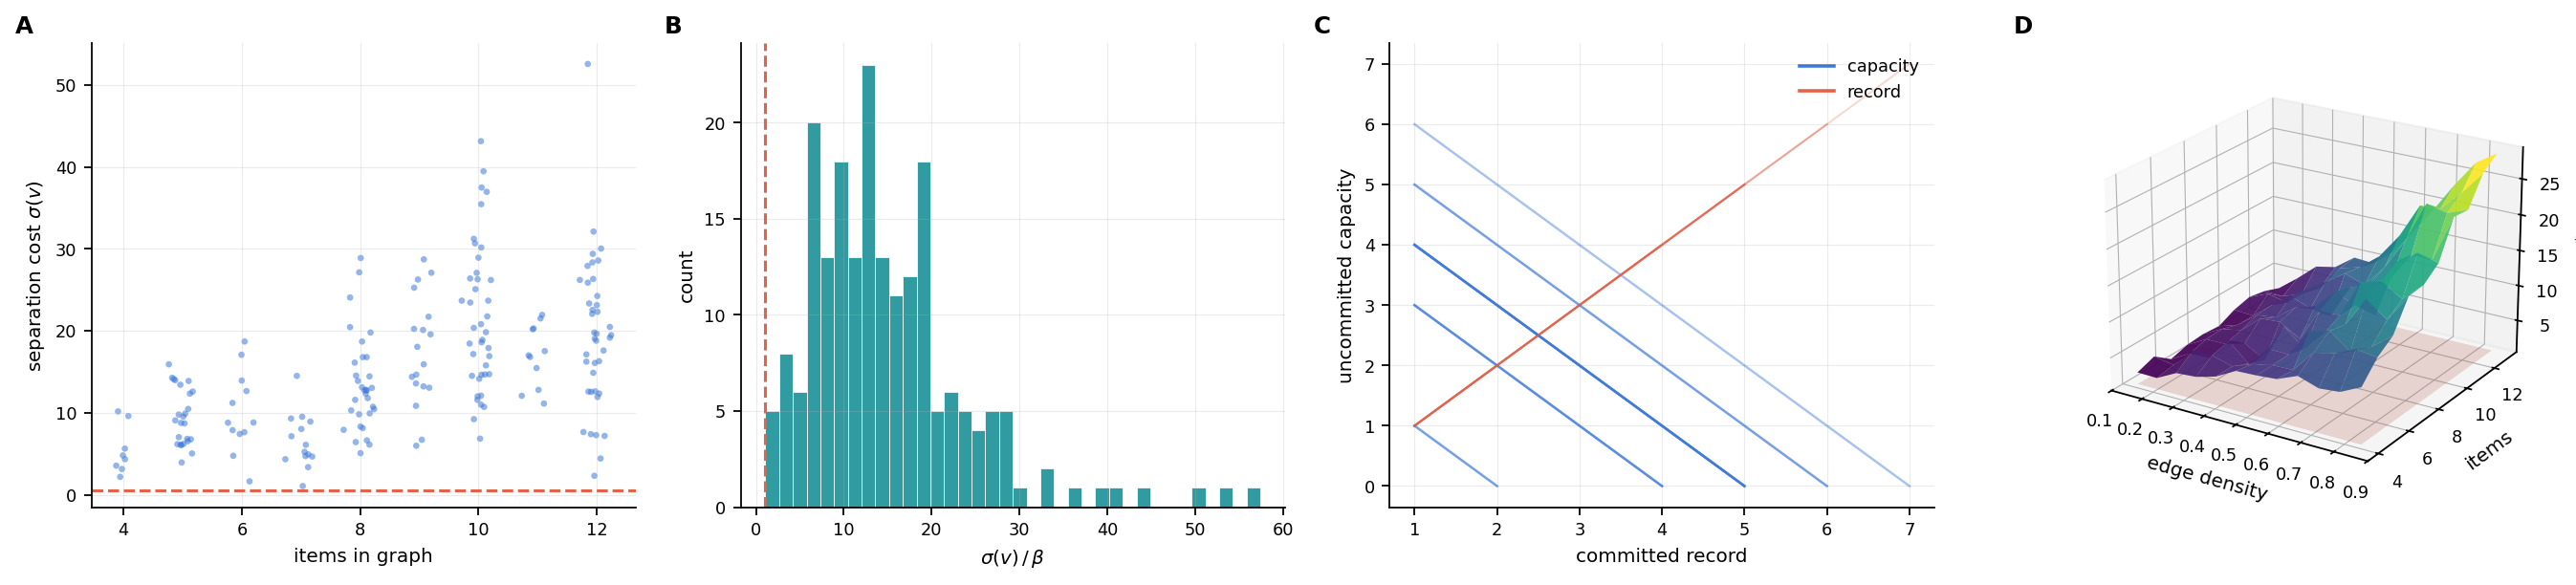
\includegraphics[width=\textwidth]{figures/panel_1_floor_blunting.png}
    \caption{\textbf{The Floor Is Positive and Every Act Consumes the
    Instrument.}
    (\textbf{A})~Separation cost $\str(v)$ on the linear $y$-axis versus the
    number of items in the graph on the linear $x$-axis ($4$ to $12$), for all
    $489$ realised separations drawn from $60$ random contact graphs at floors
    $\flo\in\{0.5,1.0,2.0\}$; points are jittered horizontally to separate
    graphs of equal size. The crimson dashed line is the floor. No point lies
    beneath it at any graph size---$0$ violations, minimum realised cost
    $0.600$---while the ceiling rises with graph size, since an item entangled
    with more others is more expensive to separate. Empirical content of
    Theorem~\ref{thm:floor} (Positive Floor).
    (\textbf{B})~Distribution of the normalised cost $\str(v)/\flo$ on the
    linear $x$-axis ($1$ to $57.4$), $36$ bins, over the same $489$
    separations. The support begins at and never crosses the crimson reference
    at $1$; the mass concentrated just above it is the population of items
    individuated by a single contact, the cheapest genuine separation, and the
    long right tail is the population individuated only by triangulating many
    weak contacts.
    (\textbf{C})~The self-blunting trajectories of Theorem~\ref{thm:blunt} for
    fourteen instruments: uncommitted capacity on the linear $y$-axis versus
    committed record on the linear $x$-axis. Capacity (steel) falls by exactly
    one and the record (crimson) rises by exactly one at every contact
    operation, the two crossing as capacity is spent. All $30$ tested
    instruments are strictly blunted and all $30$ exhibit the crossing; none
    escapes either movement.
    (\textbf{D})~Realised system floor $\flo^{\ast}$ as a three-dimensional
    surface (viridis) over edge density on the $x$-axis ($0.15$ to $0.85$) and
    item count on the $y$-axis ($4$ to $13$), each cell the mean of six random
    graphs, viewing angle elevation $22^{\circ}$ azimuth $-58^{\circ}$. The
    translucent crimson plane beneath is $\flo=1$. The surface lies above the
    plane at every density and every size, rising with both: the floor is a
    trace the non-completable medium leaves on every finite part
    (Remark~\ref{rem:floor-fact}), not an artefact of a particular graph.}
    \label{fig:panel1}
\end{figure*}


% ---------------------------------------------------------------------
%  PANEL 2
% ---------------------------------------------------------------------
\begin{figure*}[!htbp]
    \centering
    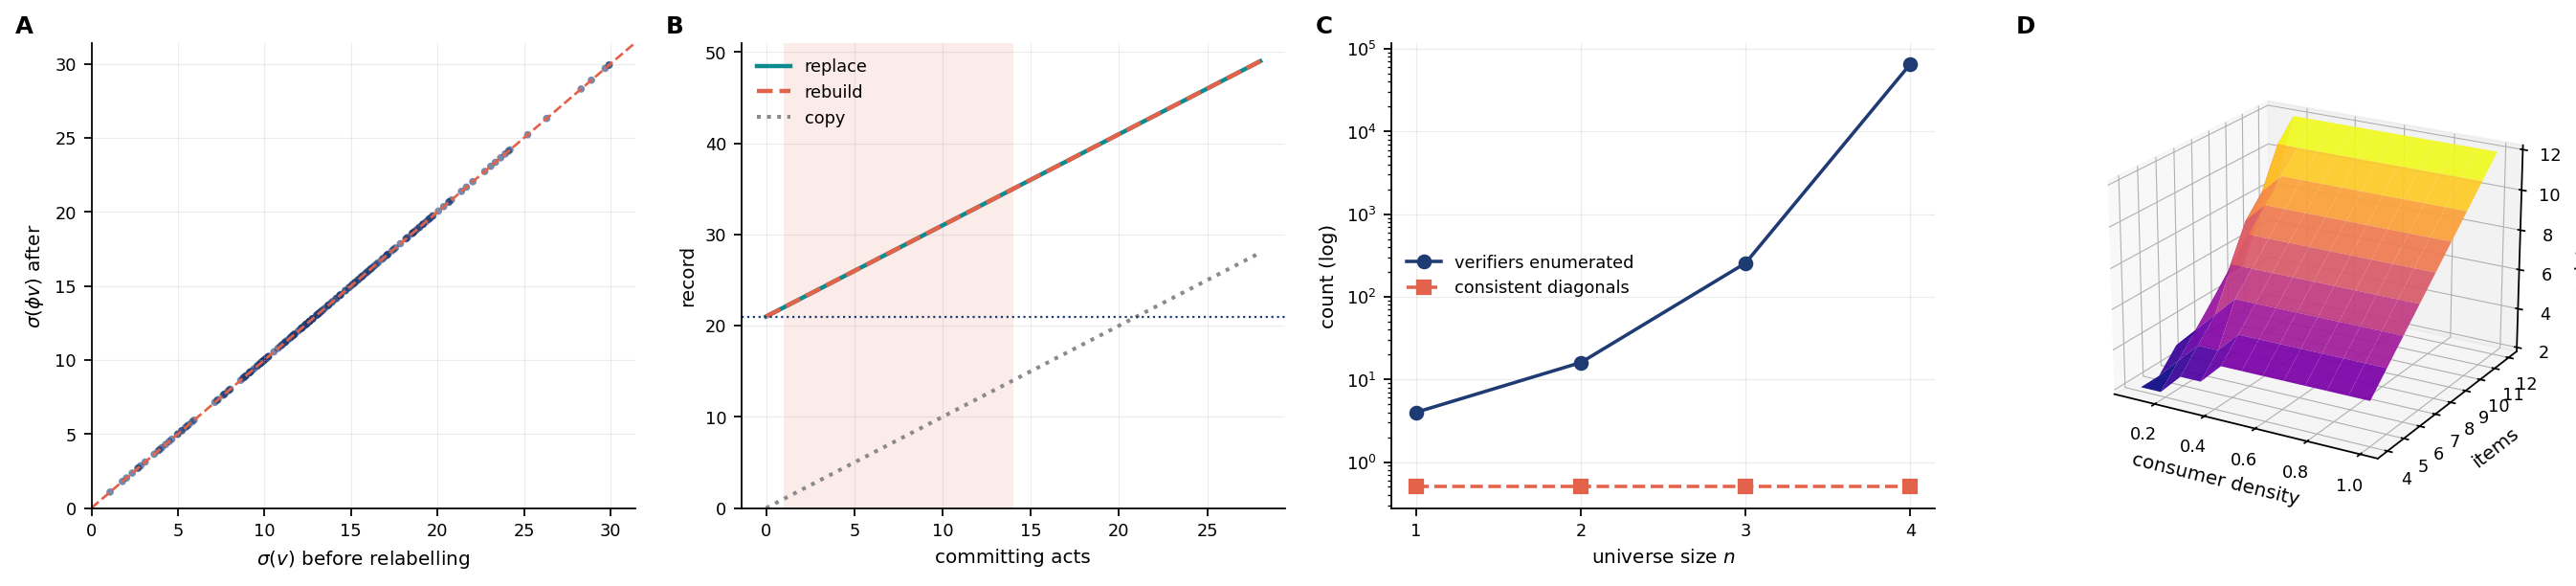
\includegraphics[width=\textwidth]{figures/panel_2_identity.png}
    \caption{\textbf{The Invariant Is Conserved; the Record and the
    Termination Condition Are What Separate Individuals.}
    (\textbf{A})~Separation cost after a random weighted relabelling on the
    linear $y$-axis versus the cost before on the linear $x$-axis, for all
    $423$ items of $60$ random graphs. Every point lies exactly on the identity
    diagonal (crimson dashed): the maximum discrepancy over the whole
    population is $0$, while $365$ of the $423$ labels were moved by the
    permutation. The datum the relabelling fixes and the datum it moves are
    plotted on the same instances---empirical content of
    Theorem~\ref{thm:invariant} (Conserved Invariant).
    (\textbf{B})~Record trajectories for the three cases of
    Theorem~\ref{thm:termination-crit} on a seven-plank structure: committed
    record on the linear $y$-axis versus committing acts on the linear
    $x$-axis. Gradual replacement (teal) and disassembly-then-reconstruction
    (crimson dashed) climb identically and share the same $\Char$; the shaded
    interval is the stage at which the reconstructed structure is \emph{open}
    in the sense of Definition~\ref{def:terminated}, which is what makes it a
    distinct individual. The copy (grey dotted) climbs on a separate lineage
    from zero. The navy reference is the record at which construction
    completed. $\Char$ is preserved in all three cases; only the record chain
    and the open stage discriminate.
    (\textbf{C})~The diagonal of Theorem~\ref{thm:self-diagonal}, enumerated
    exhaustively: total verifiers on a universe of size $n$ (navy, $2^{2^{n}}$,
    reaching $65{,}536$ at $n=4$) against the number admitting a consistent
    diagonal value (crimson squares), both on a log $y$-axis versus $n$ on the
    linear $x$-axis ($1$ to $4$). The crimson series is identically zero at
    every $n$; a single consistent case anywhere in the enumeration would
    falsify the theorem. This is a proof by exhaustion over the stated finite
    domain, not a sampled test.
    (\textbf{D})~The cell an item registers, as a three-dimensional surface
    (plasma) over consumer density on the $x$-axis ($0.1$ to $1.0$) and item
    count on the $y$-axis ($4$ to $12$), elevation $21^{\circ}$ azimuth
    $-60^{\circ}$. The same item registers a thin cell in a sparse consumer and
    a rich one in a dense consumer; across $40$ paired trials the registrations
    differed in every case and both attained their own graph's floor in every
    case. No registration is privileged---the geometry of
    Theorem~\ref{thm:receiver} (Consumer-Relativity).}
    \label{fig:panel2}
\end{figure*}


% ---------------------------------------------------------------------
%  PANEL 3
% ---------------------------------------------------------------------
\begin{figure*}[!htbp]
    \centering
    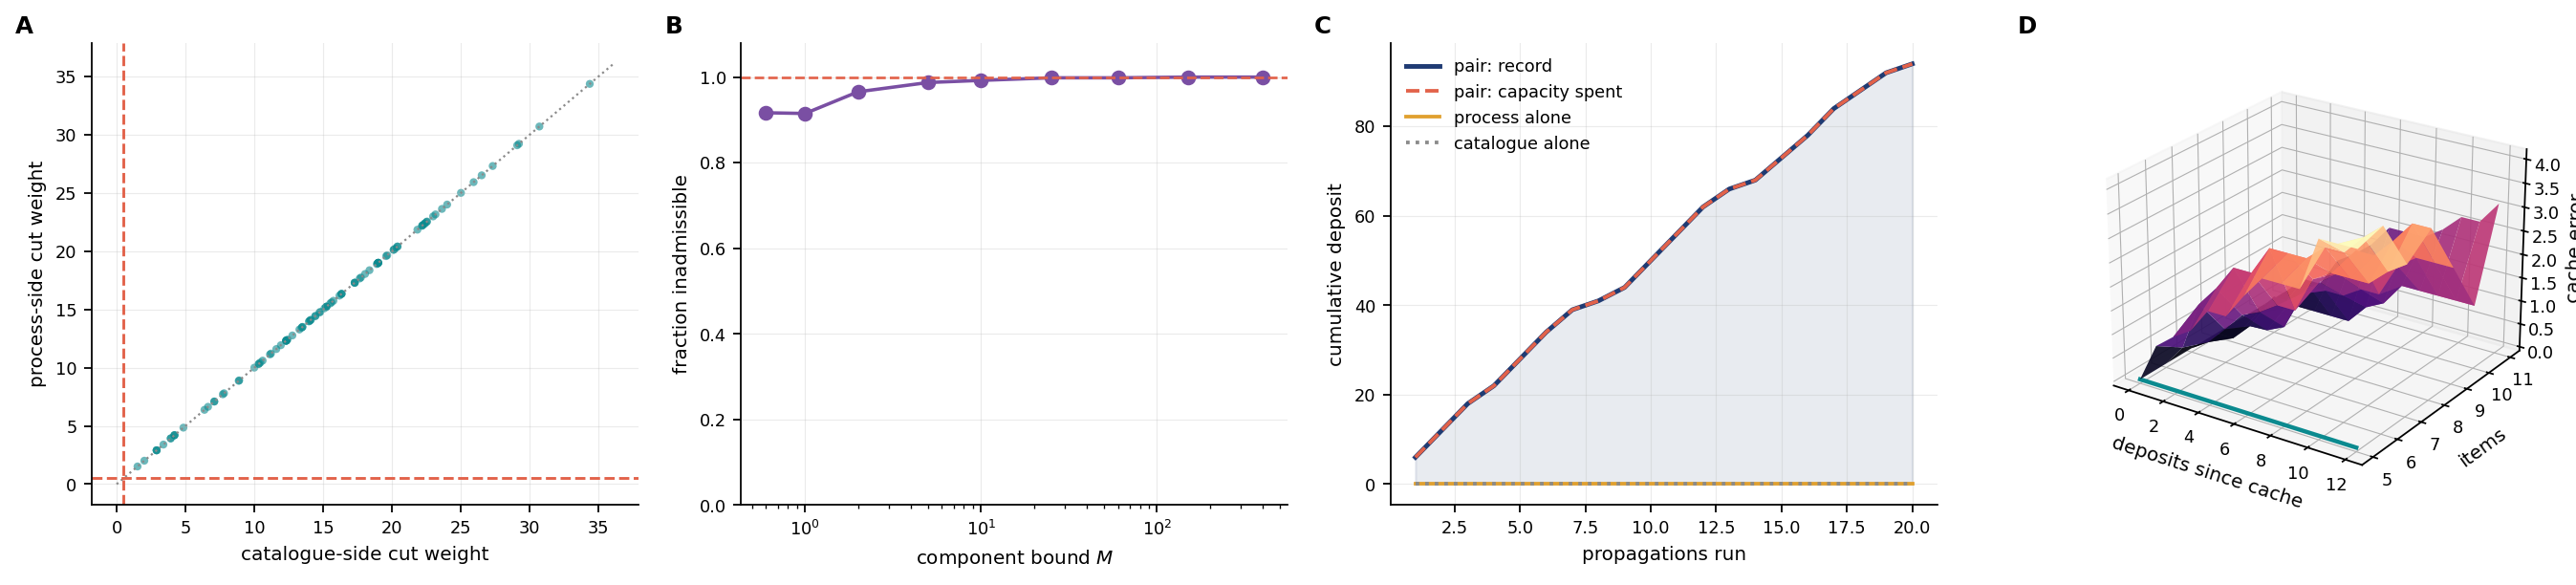
\includegraphics[width=\textwidth]{figures/panel_3_directional.png}
    \caption{\textbf{One Table, Two Directions; and the Deposit That Makes the
    Pair an Individual.}
    (\textbf{A})~Process-side cut weight on the linear $y$-axis versus
    catalogue-side cut weight on the linear $x$-axis, for $200$ outputs drawn
    from $50$ graphs, with the floor marked on both axes (crimson dashed) and
    the identity diagonal in grey. Every output of both regimes is a cut of
    weight $\ge\flo$: $0$ type violations. The two regimes do not merely
    interoperate---they return objects of one type, which is the converse half
    of Theorem~\ref{thm:catalogue-table} (Directional Identity). The forward
    half is verified separately on all $320$ items of the same graphs, with $0$
    mismatches.
    (\textbf{B})~Fraction of admissible representations carrying at least one
    component outside the range a single admissible item could occupy, on the
    linear $y$-axis versus the component bound $M$ on a log $x$-axis ($0.6$ to
    $400$), $3000$ draws per point. The fraction climbs to and remains at $1.0$
    (crimson reference) once $M$ exceeds a few units: inadmissible components
    are the generic case, not an exception, exactly as
    Remark~\ref{rem:virtual-components} asserts. Over $200$ independent trials
    the mean is preserved to a maximum error of $5.0\times10^{-15}$ while
    $98.5\%$ of representations carry an inadmissible component.
    (\textbf{C})~Cumulative deposit on the linear $y$-axis versus propagations
    run on the linear $x$-axis. The pair's record (navy) and consumed capacity
    (crimson dashed) rise together across the run; the process alone (amber)
    and the catalogue alone (grey dotted) remain flat at zero. The shaded band
    between them is what Theorem~\ref{thm:pair-blunts} supplies and neither
    half supplies on its own; the pattern held in all $40$ trials.
    (\textbf{D})~Error of a cached determination as a three-dimensional surface
    (magma) over deposits since caching on the $x$-axis ($0$ to $12$) and item
    count on the $y$-axis ($5$ to $11$), elevation $24^{\circ}$ azimuth
    $-56^{\circ}$. The surface rises away from the teal zero-line, which is the
    pair recomputing against the current graph. Across $40$ trials the cache
    went stale in $21$ and the pair in $0$: the geometry of
    Proposition~\ref{prop:staleness} against
    Corollary~\ref{cor:no-staleness}.}
    \label{fig:panel3}
\end{figure*}


% ---------------------------------------------------------------------
%  PANEL 4
% ---------------------------------------------------------------------
\begin{figure*}[!htbp]
    \centering
    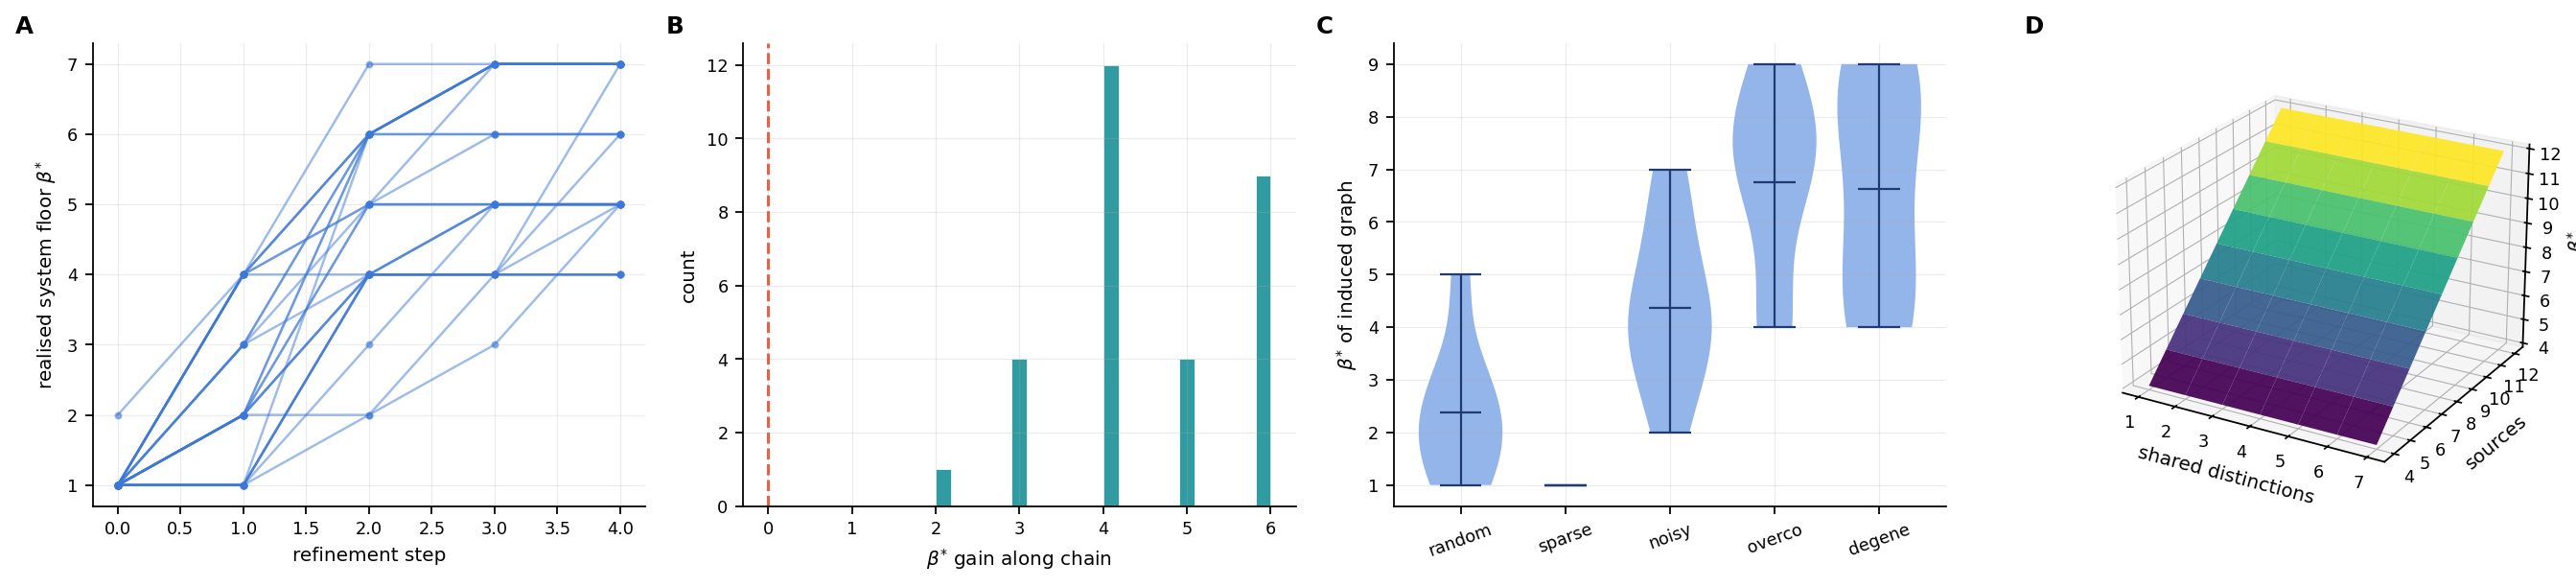
\includegraphics[width=\textwidth]{figures/panel_4_construction.png}
    \caption{\textbf{The Calculus Is Indifferent to the Quality of the Term
    Map, and the Realised Floor Reports That Quality Without a Reference.}
    (\textbf{A})~Realised system floor $\flo^{\ast}$ on the linear $y$-axis
    versus refinement step on the linear $x$-axis ($0$ to $4$), for $26$ of the
    $40$ chains of term maps ordered by the refinement relation of
    Definition~\ref{def:refinement}. Every chain is monotone non-decreasing;
    across all $40$ valid chains there are $0$ monotonicity violations. This is
    the empirical content of Theorem~\ref{thm:floor-readout} (Floor
    Monotonicity).
    (\textbf{B})~Distribution of the floor gain from the coarsest to the finest
    map of each chain, $22$ bins, with the crimson reference at zero. The
    support lies entirely to the right of it: no chain loses floor under
    refinement, and the gains cluster at $4$ to $6$ units.
    (\textbf{C})~Distribution of the realised floor by kind of term map, as
    violins over five deliberately adversarial families---random, sparse,
    noisy, over-connected, and degenerate (every source drawing identical
    distinctions), $60$ maps in total. Every family induces a graph on which
    the floor, the edge bound, relabelling invariance, and cut non-emptiness
    all hold: $0$ failures, the content of Theorem~\ref{thm:tau-agnostic}. The
    families differ markedly in the floor they induce, which is the coarsening
    of Corollary~\ref{cor:coarsen} made visible. Note that the degenerate
    family induces among the \emph{highest} floors while discriminating worst:
    the floor is a monotone signal of refinement, not a quantity to maximise
    (Remark~\ref{rem:quality-honest}).
    (\textbf{D})~Realised floor as a three-dimensional surface (viridis) over
    the number of shared distinctions on the $x$-axis ($1$ to $7$) and the
    number of sources on the $y$-axis ($4$ to $12$), each cell the mean of five
    induced graphs, elevation $23^{\circ}$ azimuth $-60^{\circ}$. The surface
    is smooth and monotone in the shared-distinction axis: more shared
    structure yields a higher floor and correspondingly coarser cells, across
    the whole two-dimensional parameter region.}
    \label{fig:panel4}
\end{figure*}


% ---------------------------------------------------------------------
%  PANEL 5
% ---------------------------------------------------------------------
\begin{figure*}[!htbp]
    \centering
    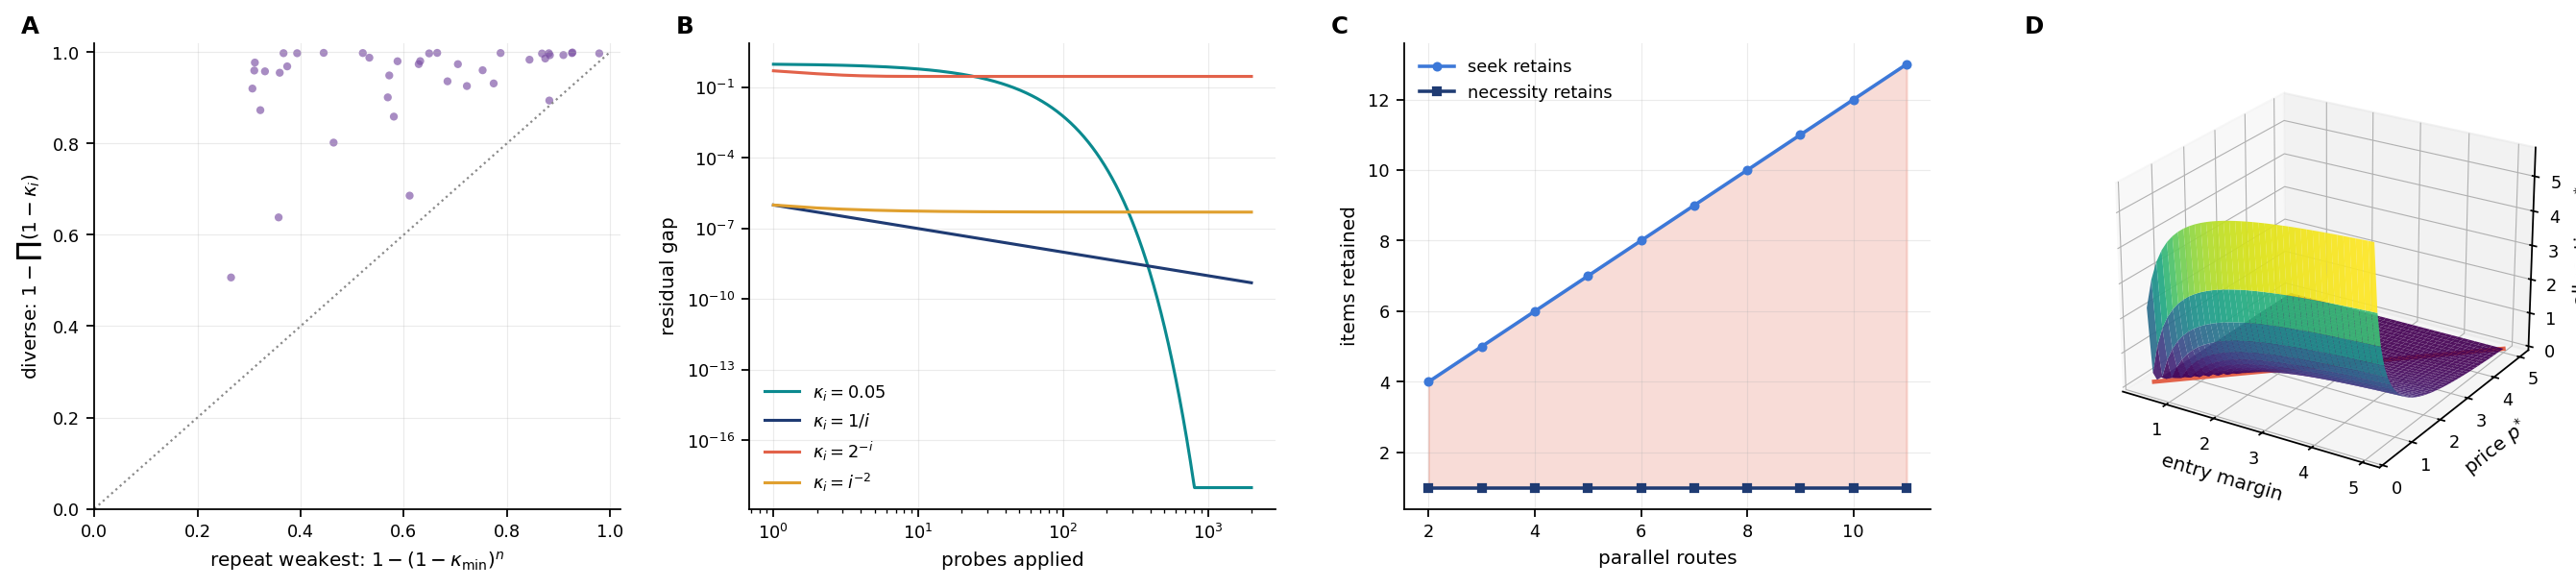
\includegraphics[width=\textwidth]{figures/panel_5_probing.png}
    \caption{\textbf{Probes Compound Rather Than Vote, Saturate Only Under a
    Divergent Sum, and Divide a Budget at a Single Price.}
    (\textbf{A})~Composite power of a chain of distinct probes,
    $1-\prod_i(1-\pot_i)$, on the linear $y$-axis versus the composite power of
    repeating its weakest member the same number of times,
    $1-(1-\pot_{\min})^{n}$, on the linear $x$-axis, over $300$ instances with
    the identity diagonal in grey. Every point lies strictly above the
    diagonal---$300$ of $300$, with no ties---so diversification strictly
    dominates repetition (Corollary~\ref{cor:diversify}). The underlying
    composition law is verified separately on $400$ chains to a maximum
    absolute error of $1.1\times10^{-16}$ (Theorem~\ref{thm:multiplicative}).
    (\textbf{B})~Residual gap on a log $y$-axis versus probes applied on a log
    $x$-axis ($1$ to $2000$), for four canonical power sequences. The two with
    divergent sums---constant $\pot_i=0.05$ (teal) and harmonic $\pot_i=1/i$
    (navy)---drive the residual toward zero; the two with convergent
    sums---geometric $\pot_i=2^{-i}$ (crimson) and inverse-square
    $\pot_i=i^{-2}$ (amber)---plateau strictly above it and stay there. At a
    horizon of $4000$ probes all four sequences match the prediction of
    Corollary~\ref{cor:saturation}: $0$ mismatches.
    (\textbf{C})~Items retained on the linear $y$-axis versus parallel routes
    on the linear $x$-axis ($2$ to $11$), on the diamond witness of
    Theorem~\ref{thm:separation-operators}. The $\seek$ operator (steel) climbs
    linearly from $4$ to $13$ while $\nec$ (navy) stays flat at $1$; the shaded
    region between them is the over-retention a reachability-only mechanism
    incurs, growing from $3$ to $12$ items. On the chain witness the
    complementary identity holds at every tested length: every interior item is
    necessary and the terminal leaf is reachable yet redundant. Over $60$
    random graphs the containment $\nec\subseteq\reach$ holds without
    exception, with a strictly positive gap in $57$, and necessity coincides
    with domination on all $211$ non-seed items checked
    (Corollary~\ref{cor:no-single}).
    (\textbf{D})~Optimal allocation $a_i^{\star}$ as a three-dimensional
    surface (viridis) over entry margin $\gain_i'(0)$ on the $x$-axis ($0.4$ to
    $5.0$) and shadow price $\price$ on the $y$-axis ($0.25$ to $5.0$),
    elevation $24^{\circ}$ azimuth $-58^{\circ}$. The surface rises with margin
    and falls with price, collapsing to the zero floor along the crimson line
    where the entry margin meets the price---the sharp dropout boundary of
    Theorem~\ref{thm:waterfill}. Across $120$ convex instances the stationarity
    conditions hold, the budget is respected, the dropout boundary is sharp,
    and the price is nonincreasing in the budget and nondecreasing in the probe
    count, in $120$ of $120$ cases each.}
    \label{fig:panel5}
\end{figure*}


% ---------------------------------------------------------------------
%  PANEL 6
% ---------------------------------------------------------------------
\begin{figure*}[!htbp]
    \centering
    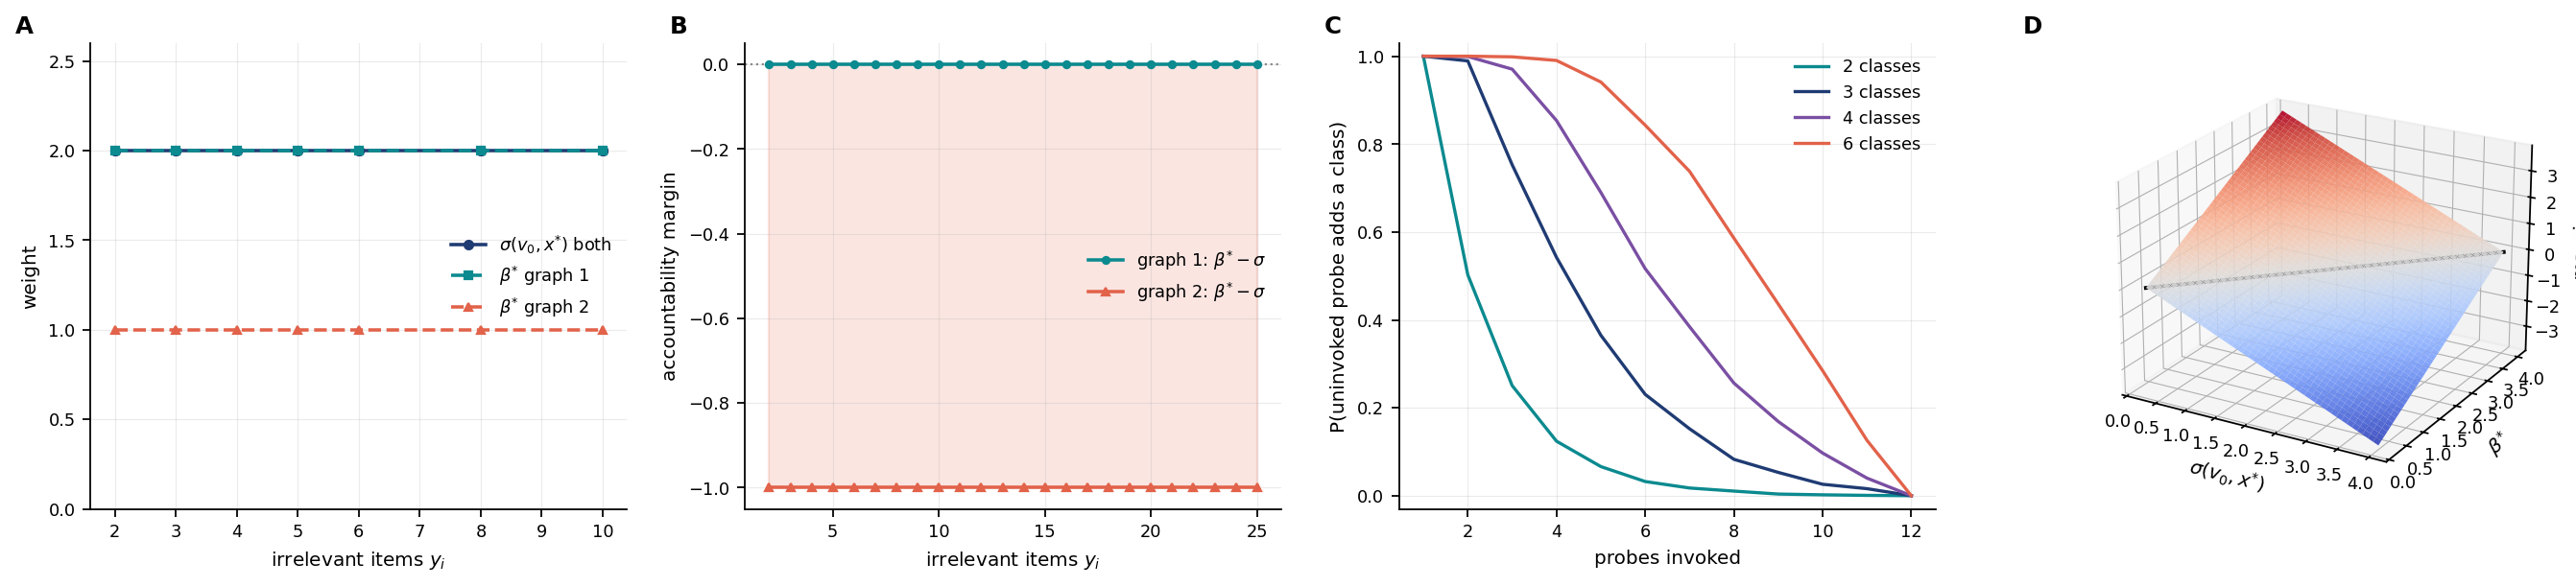
\includegraphics[width=\textwidth]{figures/panel_6_separation.png}
    \caption{\textbf{The Verdict Is a Global Quantity, and the Witness Is
    Invisible to Every Local One.}
    (\textbf{A})~The witness pair of Theorem~\ref{thm:query-separation} as the
    number of irrelevant items $y_i$ grows along the linear $x$-axis ($2$ to
    $10$), weights on the linear $y$-axis. The pair alignment
    $\str(v_0,x^{\star})$ is identical in the two graphs (navy, filled and open
    markers coincident at exactly $2.0$), while the system floors separate:
    $2.0$ in graph~1 (teal) against $1.0$ in graph~2 (crimson). The two graphs
    have identical contact relations at every size---the same assertion set,
    hence identical under every retrieval query---yet the verdicts differ at
    $\eps=0$.
    (\textbf{B})~The accountability margin $\flo^{\ast}-\str(v_0,x^{\star})$ on
    the linear $y$-axis, swept to $25$ irrelevant items on the linear $x$-axis.
    Graph~1 sits at exactly $0$ (accountable, teal) and graph~2 at exactly
    $-1$ (not accountable, crimson), the two shaded to the zero reference and
    both flat: adding items that lie on no path between the queried pair moves
    the verdict without moving anything local to it. This isolates the
    asymmetry of Remark~\ref{rem:separation-meaning}---the queried quantity is
    local and equal, the threshold is global and different. A bounded pattern
    confined to the queried pair's neighbourhood is fooled in $200$ of $200$
    instances (Corollary~\ref{cor:attributed}), and none of $500$
    corpus-determined maps spanning five families separates the two graphs
    (Theorem~\ref{thm:corpus-separation}).
    (\textbf{C})~Probability that an uninvoked probe still reaches a new
    equivalence class, on the linear $y$-axis ($0$ to $1$), versus probes
    already invoked on the linear $x$-axis ($1$ to $12$), for registries
    admitting two, three, four, and six classes, $4000$ draws per point. A
    fixed confidence criterion is satisfied at the first probe while this
    probability remains near unity, and it decays only as the registry is
    exhausted---the content of Theorem~\ref{thm:closure-stronger} (Closure Is
    Strictly Stronger). Over $300$ runs to closure, $169$ terminated in
    convergent closure and $131$ in contested closure, with none running on
    (Theorem~\ref{thm:decline}).
    (\textbf{D})~The verdict surface: the accountability margin as a
    three-dimensional surface (coolwarm) over the pair alignment
    $\str(v_0,x^{\star})$ on the $x$-axis and the system floor $\flo^{\ast}$ on
    the $y$-axis, both $0.2$ to $4.0$, at $\eps=0$, elevation $22^{\circ}$
    azimuth $-60^{\circ}$. The black line is the decision boundary
    $\str=\flo^{\ast}$, above which a determination is accountable and below
    which it is not. The two witness graphs sit on opposite sides of this
    boundary while agreeing on every quantity a store of assertions records;
    the pair decides the verdict correctly on $200$ of $200$ random instances
    and separates the witness that no corpus-determined map separates
    (Theorem~\ref{thm:pair-expresses}).}
    \label{fig:panel6}
\end{figure*}
